\subsection{Earlier utility aggregates and operating measurements}\label{app:earlier-operating-records}

The earlier detailed summaries in \cref{fig:fw-trainval} cover only 25 rounds. In that subset,
training utility exceeds validation utility by 0.282--0.290
(\cref{fig:fw-trainval}). This is a difference between reported aggregates
on separate training and validation contexts; it does not isolate a cause
or establish behavior in the missing summaries. The late validation plateau
is evidence to explain, rather than proof of useful transfer. Encoder
integrity and parameter updates require their own receipts; the plotted
utility tables do not establish either.

\begin{figure*}[!t]
  \setlength{\abovecaptionskip}{4pt}
  \centering
  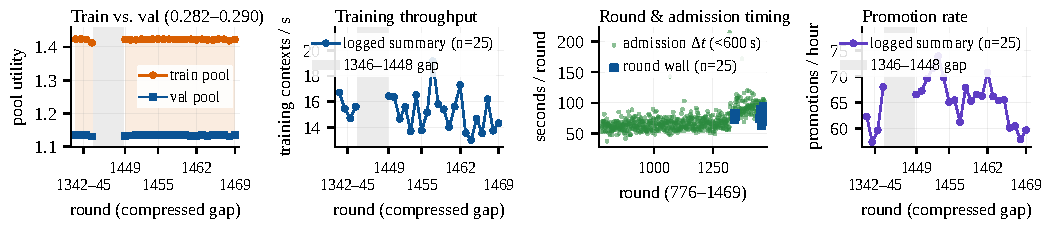
\includegraphics[width=\linewidth,height=1.50in,keepaspectratio]{figures/fig_fw_telemetry.pdf}
  \caption{\textbf{Train--validation aggregates and operating measurements from earlier retained windows.}
  First, second and fourth panels: 25 retained summaries spanning rounds 1342--1345 and 1449--1469
  (rounds 1346--1448 were not retained), showing train versus validation pool utility (gap 0.282--0.290),
  distinct training contexts per completed-round second and strict training-program promotions per hour
  over up to 20 completed rounds including qualification waits. Third panel: consecutive admission-timestamp
  intervals: all 695 admission rows (775--1469) carry timestamps, giving 694 consecutive pairs.
  The panel plots the 692 positive differences below 600\,s (green), excluding two longer pauses,
  alongside the 25 measured round wall times (blue squares).
  Scope: \cref{sec:method-status}.}
  \label{fig:fw-telemetry}
  \label{fig:fw-trainval}
\end{figure*}

\paragraph{Retained operating windows.}
In the five earlier 20-round program-event slices, rounds 2005--2024 record 15
events (\cref{fig:fw-recent-development}), rounds 2082--2101 record 10
(\cref{fig:fw-followup-development}), rounds 2343--2362 record 22
(\cref{fig:fw-later-development}), rounds 2508--2527 record 15
(\cref{fig:fw-subsequent-window}), and rounds 2644--2663 record 21
(\cref{fig:fw-program-promotions}). Each slice records zero adapter admissions.
The later 20-round throughput slice, 2696--2715, also records none; it
reports contexts and wall time rather than a program-event total.
Completed-time, event-distribution and rate summaries appear in
\cref{app:development-time,app:event-counts,app:subsequent-rates,app:promotions-per-hour,app:round-throughput}.
Scope and clock definitions follow \cref{sec:method-status}.
